\section{Fundamentals of \eu}
\label{sec:basics}

\paragraph {A brief note on \eu history and notation} The origin of
what we will call \eu in this chapter, is derived from the
\texttt{HSTS} planner \cite{mus94} used on a number of ground-based
demonstrations for space telescope scheduling as noted in Section
\ref{sec:rabeyond}. \texttt{HSTS} was also the
\texttt{LISP}-based\footnote{This was the first (and to our knowledge
  only) software ever to been written in \texttt{LISP} to be flown in
  space.} planner that was flown as part of the Remote Agent
\texttt{RAX} experiment. Concurrent to \texttt{RAX} deployment, a C++
version of the planner was implemented which went on to be used for
the \texttt{MAPGEN} \cite{bresina05} system and continues to be used
to date, in the mission-critical uplink process for the
command/control of the Mars Exploration Rovers (\texttt{MER})
mission. A vastly re-factored, higher performance open source version
\cite{europapso} was named \eut and is the subject of this chapter and
used by \rx.  Note however, in using the name \eu, we refer to the
\emph{fundamental ideas as well as the planning paradigm} even if
there exists a specific implementation.

\subsection{Introduction}
\label{sec:euintro}

\eu uses a \emph{domain model} written in a declarative language,
together with initial conditions and goals (also in that specified
language), to construct a set of temporal relations that must be true
at start time. These models include assertions about the physics of
the vehicle, i.e how it responds to external stimulus and internally
driven goals. By propagating these relations forward using Simple
Temporal Networks \cite{dechter91} and applying goal constraints, \eu
can select a set of conditions that should be true in the future,
where some of these conditions will correspond to actions the agent
must take. The planner can backtrack and try another path during the
search process if a goal cannot be reached while being capable of
discarding unachievable goals.

Traditionally robot execution has relied on dispatching commands at
precise times. Such linear sequences of precisely timed commands give
no ability to adjust execution on the basis of sensory
information. Although some commands can issue tests on sensor
readings, these tests have the objective of verifying whether expected
execution conditions are occuring. If not, the state of the system is
declared off-nominal and execution of the sequence of commands is
interrupted. More recently, executives have been proposed and
implemented that significantly broaden the way robots can be commanded
\cite{mus98,alami:1998p820}. For example, the Remote Agent executive
interpreted a \textit{temporally flexible plan} which represents each
start time as a variable and contains an explicit network of bounded
delay constraints between such
variables. Fig. \ref{fig:flex-timelines} shows an example of a
flexible partial plan.

\begin{figure}[!htb]
\centering
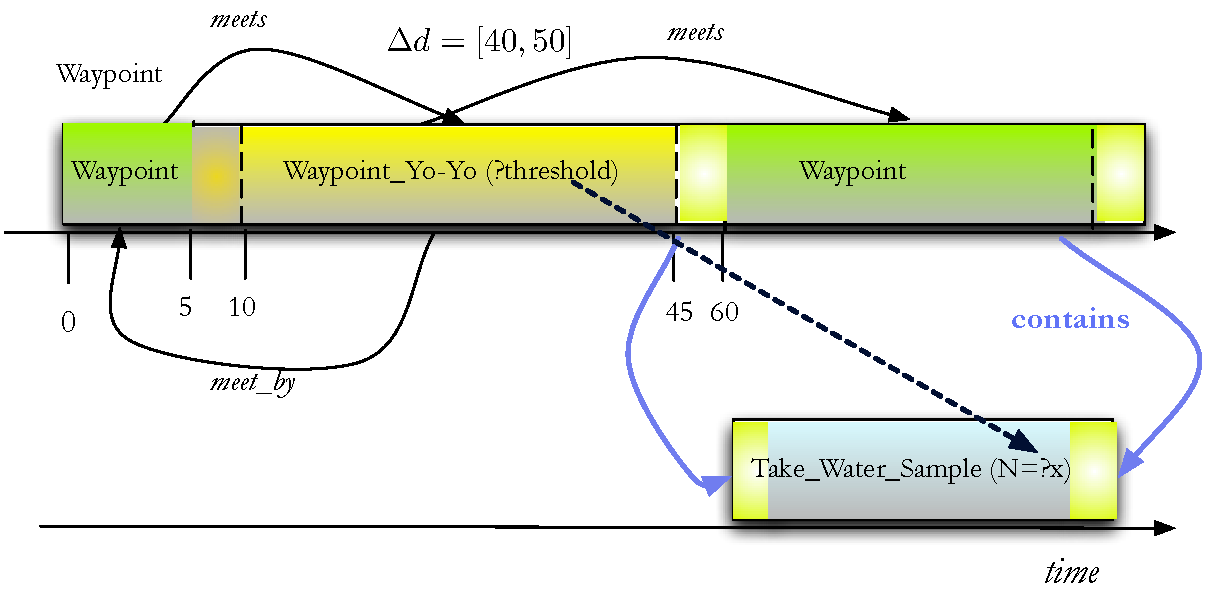
\includegraphics[scale=0.35]{figs/flexible-timelines.pdf}
\caption{\small Tokens with flexible temporal intervals and parametric
  constraints between tokens. This example shows the triggering of a
  water sampler based on a feature threshold while the vehicle
  Yo-Yo's. The \texttt{Waypoint\_Yo-Yo} token has a flexible duration,
  start \& end times.}
\label{fig:flex-timelines}
\end{figure}

Unlike a traditional fixed time-tagged command sequences, such
flexible plans leave room for adaptation at execution time. When the
executive considers when to start a task, it propagates information
through the constraint network, computes a time bound for the
variable, selects an actual execution time within the bound, and
starts the task at that time. Temporally flexible plans therefore,
express a \textit{range of possible outcomes} of the robots
interaction with the environment within which the executive can elect
at run time, the most appropriate for actual execution. The fact that
constraints are explicitly represented ensures that through constraint
propagation the executive will respect global limits expressed in the
plan (e.g., don't start a task until a certain condition has been
satisfied but still satisfying some overall deadline). Such
flexibility is critical when dealing with dynamic and uncertain
conditions such as in the ocean, where precise timing of a robotic
action might be indeterminate. Further, the advantage of flexibility
can be contrasted with the consequences of the intrinsic inflexibility
of traditional command sequences. Because they are inflexible,
sequences must necessarily be designed considering worst case
scenarios.

\eu uses a \emph{state variable} representation
\cite{mus94,jonsson00,mcgann09} to describe the evolution of state
over time. The instantiated history of such state variable evolution
over a temporal horizon we call \emph{timelines} and which represent a
single thread in the execution of a concurrent system. At any given
time each thread can execute a single procedure.  Thus each timeline
consists of a sequence of procedures which encapsulate and describe
state evolution; we call these instantiated atomic entities
\emph{tokens}.  A token therefore describes a procedure invocation,
the state variables on which it can occur, the parameter values of the
procedure, and the time values defining the interval. We allow
encapsulation of uncertainty within these tokens with a range of start
and end times and parameters, all of which are encoded as variables. A
constraint solver in turn manipulates these variables defined in a \eu
domain model. For example, consider a scientific need to take water
samples 100 meters from an environmental hotspot while an AUV is
performing a Yo-Yo sawtooth pattern in the water-column. Two samples
are needed if the feature's signal is above a threshold; one
otherwise. The token that is capturing the sensory threshold has a
parametric constraints to the token which fires the requisite water
sampler. In addition, the start time of the water sampling procedure
is highly dependant on the variability of sub-sea currents and actual
speed of the vehicle. Therefore a number of values are possible for
the start times and duration of the sampling all of which are valid
combinations for desired outcomes.

\subsection{\eu Plan Representation}
\label{sec:europa:pr}

\eu follows the representation outlined by the \texttt{CAIP} framework
augmenting with elements that are necessary for an efficient
implementation of constraint-based planning. Below we describe briefly
the main elements, followed by a detailed description for each of
these elements and how together they constitute a rich
representational paradigm for inference in Sections
\ref{sec:europa:modeling}, \ref{sec:europa:inference} and
\ref{sec:europa:search}.

\begin{enumerate}

\item \textbf{Tokens} Temporally scoped entities that correspond to
  Intervals in the \texttt{CAIP} framework, are used to represent
  state and actions in time. A\textbf{Token State model} is defined to
  support an efficient implementation of plan-space search algorithms.

\item \textbf{Domains, Variables and Constraint} are used to represent
  restrictions in the problem domain in terms of a \texttt{CP}
  formulation.

\item \textbf{Domain Rules} are used to describe internal and external
  relationships on and between tokens, as presecribed by
  \texttt{CAIP}.
  
\item \textbf{Objects} are used to represent problem domains in a more
  modular and scaleable way. \textbf{Timelines and Resources} are
  built in implementations of Object types that appear frequently in
  real-world domains.

\end{enumerate}

At the atomic level, the entities in the \eu plan representation are:

\begin{description}

\item[\textbf{Variables}] Values that need to be represented to
  describe the problem domain and over which we may want to specify
  constraints. In the Shopping Agent example, the times at which the
  agent needs to leave or be back, or executes a purchase, are all
  instances where variables representing time is used.  As noted in
  Section \ref{sec:europa:cp}, a variable can take values from a
  domain. In \eu, domains are defined over a specific data type, the
  primitive data types supported are, \textit{String},
  \textit{Boolean}, \textit{Numeric} and \textit{Object} (see
  below). Further, two types of variable Domains can be defined over a
  data type, \textit{Enumerated} and \textit{Interval} (used only for
  numeric data types, they are specified by a [LowerBound,UpperBound]
  pair, for instance: [1,10], [5.0,100.0]). It is this latter ability
  to represent and reason over numeric intervals that forms the basis
  of representing flexible plans.

\item[\textbf{Constraints}] valid plans in most problem domains have
  to satisfy a number of restrictions, for instance, a Shopping Agent
  may only be able to perform one task at a time, may have limited
  time or an energy or fuel budget to perform a task. In \eu, these
  restrictions are represented by constraints, which can be defined
  over any combination of variables in a domain. \eu provides a
  \emph{Constraint Library} that implements a number of useful
  constraints (temporal, resource, relational), while allowing the
  possibility to add new constraints if required by a particular
  domain.

\item[\textbf{Objects}] The items we wish to describe and refer to in
  a domain are considered objects. As in the case with object-oriented
  analysis and design, one can seek out the nouns in any domain
  description to find likely objects. In the Shopping Agent example,
  we might consider the Agent, Products and Locations all to be
  objects. Objects have state and behavior, for example, a Shopping
  Agent can have, its location, a bag that contains the products it
  has already purchased (the bag can in turn be another object) and
  behavior as in going to a location to look for a product, perform a
  purchase, return home, etc.

  Objects that have similar state and behavior can be described
  generically in terms of object types or classes. \eu allows the
  definition of classes similar to object-oriented programming
  languages, where a class can have attributes (represented by
  variables), and classes can be arranged in a single-parent hierarchy
  through inheritance.  However, one key aspect in \eu that is not
  found in object-oriented programming: to describe state and behavior
  for the purposes of planning we need to build on the formalism of
  first order logic.

\item[\textbf{Tokens}] In first order logic, a predicate defines a
  relation between objects and properties \cite{gen87}.  In \eu, we
  define such relations between variables whose domains are sets of
  objects and sets of properties to describe state and behavior. For
  example, one might use a predicate \texttt{At($a$,$l$)} to indicate
  that agent $a$ is at location $l$, or a predicate
  \texttt{Buy($a$,$p$}) to indicate that agent $a$ is taking action to
  buy product $p$. Note that $a$ is a variable which may have a number
  of possible values in a problem with multiple agents. Similarly, $l$
  and $p$ are variables whose values are the set of possible positions
  and products respectively. \eu can be used to create partial plans,
  where the domains of variables $a$ and $l$ can have more than one
  possible value. Or they can be grounded plans, where single values
  will be specified for each variable as showing in the N-queen's
  problem.

  In general, for an executable plan it is insufficient to state
  predicates that describe required state or behavior without also
  specifying some temporal extent over which each of those predicates
  hold. Predicates that are always true can be thought to hold from
  the beginning to the end of the planning horizon. However, in
  practice, the temporal extent of interest must be defined with
  timepoints \cite{Dean88} to represent its start and end.  In such
  representation, one writes \texttt{At($a$,$s$,$e$,$l$)} to indicate
  that agent $a$ is at location $l$ from time $s$ to time $e$. In
  fact, this pattern of using such predicates to describe both state
  and behavior of objects is prevalent enough that \eu the token
  representation. Token have built in variables to indicate the object
  to which the statement principally applies as well as the timepoints
  over which it holds. A token is an instance of a predicate that
  represents an object's state or behavior and is defined over a
  temporal extent. In \eu, all predicate instances are tokens. Also,
  in the same way that objects are described generically by classes,
  in \eu tokens can be described generically by token types. Every
  token has five built-in variables:

  \begin{enumerate}

  \item \textit {start}: The beginning of the temporal extent over
    which the token predicate is defined.

  \item \textit {end}: The end of the temporal extent over which the
    predicate is defined.

  \item \textit {duration}: The duration of the temporal extent. The
    constraint \textit{start} $+$ \textit{duration} = \textit{end} is
    enforced automatically.

  \item \textit{object}: The set of objects to which a token might
    apply. In a grounded plan representation each token applies to a
    specific object, reflecting the intuition that tokens are used to
    describe some aspect of an object (\ie state or behavior) in
    time. However, in a partial plan, it is possible that the
    commitment to a specific object may not yet have been made.

  \item \textit{state}: Tokens can be \texttt{ACTIVE, INACTIVE,
      MERGED}, or \texttt{REJECTED}. The state variable captures the
    token's current state and its reachable states through further
    restriction.  This is required to support \texttt{CAIP}'s approach
    to planning where goals and subgoals can be satisfied by either
    adding new intervals (tokens) to the plan, or by merging with
    existing intervals. % Token state lifecycle is examined in detailed
    % in a separate section below.

  \end{enumerate}

\item[\textbf{Built-in Object Types}] In a domain model, there may be
  some classes that don't have any time-dependent state or behavior,
  and therefore those classes will not have any token types associated
  with them. For instance in the Shopping Agent model, the set
  locations and products are static for the agent's purposes so one
  may only want to declare them but not associate any state or
  behavior with them.  However, a common case in a non-trivial domain
  model is that objects will have many associated tokens in order to
  describe their state and behavior throughout a plan. There are some
  object types that are commonly used in domain descriptions, that \eu
  provides a built-in implementation for them:

\begin{enumerate}

\item \textit{Timelines}: Often objects in a domain must be described
  by exactly one token for every given timepoint in the plan. Any
  instances of a class derived from \eus built-in timeline class will
  induce ordering requirements among its tokens to ensure no temporal
  overlap may occur among them \cite{mus94}.  \kcomment{add a figure}

\item \textit{Resources}: Metric resources, e.g. the energy of a
  battery or the capacity of a cargo hold, are objects with an
  explicit quantitative state in time and with a circumscribed range
  of changes that can occur to impact that state i.e. produce,
  consume, use, change.  Resources are a common requirement for \eu
  users that built-in object types (with their corresponding token
  types to denote production, consumption, etc) are provided.
  Instances of classes derived from a resource will induce ordering
  requirements on their tokens in order to ensure that the level of
  the resource remains within specified limits.  \kcomment{This
    definitely needs a visual example and some text esp. since it
    impacts plan structure via scheduling}

\end{enumerate}

\item[\textbf{Token State Model}] In \eus representation, goals are
  temporally scoped states that need to be achieved, or actions that
  must be performed. As a result, \eu internally represents goals as
  tokens.  Goals can be posted explicitly, for example, when a user
  asks the Shopping Agent to own a specific product by a specific
  time, or implicitly when subgoals are created as a result of domain
  compatibilities \kcomment{Define a compatibility}. For instance,
  when the Shopping Agent must get to a location where a product is
  available before it is able to purchase it: in this case the
  original goal of purchasing the product spawns a subgoal of being at
  a specific location without which the purchase will not occur as
  defined in the domain model.  Looking at a how a simple Shopping
  Agent goal would be addresed by \eu helps illustrate how Token
  States support the planning process.  Let's assume the planner
  starts with a partial plan that places the Shopping agent at home at
  time $0$ with no products in possession.  If a goal is posted for
  the Agent to own a drill by time 10. \kcomment{Use Fig 4 and edit::
    Add figure showing an AgentLocation timeline with an At(Home)
    token with start=0 and end open, an empty AgentBag timeline, and a
    Own(Drill) token with start=10 floating below both timelines}

  Note that the \texttt{Own(Drill)} token that represents the goal is
  not immediately placed on the \texttt{AgentBag} timeline since \eu
  must determine whether it can achieve that goal and how. When the
  goal is posted and before any decisions are made, the
  \texttt{Own(Drill)} token is created in an \texttt{INACTIVE}
  state. \eu then considers the partial plan and evaluates two
  possible alternatives:

\begin{enumerate}

\item If there are any tokens in the plan that are compatible with the
  new goal, \eu may attempt to satisfy the goal by \emph{merging} it
  with any of them (if there is more than one it can try them one at a
  time or in some heuristic order), in this case, the state of the
  token would change to \texttt{MERGED}.

\item Instead of merging with existing tokens in the plan, \eu may
  decide to \emph{insert} a new token into the plan, in which case the
  state would change to \texttt{ACTIVE}.

\end{enumerate}

When a token is merged, all restrictions imposed on the merged token
are transferred to the active token upon which it is merged. Merging a
token requires finding a target active token that is compatible. Two
tokens are merge-compatible if they are instances of the same
predicate and that no intersections between corresponding variables
are empty. The effect of merging is illustrated in Figure 3
\kcomment{Which figure?}.\comment{Use previous fig and modify as
  appropriately:: Add figure showing the effect of merging; all figs
  on this section are conjoined. JB to sketch it out.}

When a token is activated all compatibilities \kcomment{this should
  have been defined earlier} associated with its type are evaluated,
which may lead to new subgoals being generated. In our example, there
could be a compatibility stating that the Shopping Agent must be at
the same location as the product it is purchasing. In such a case,
activating the \texttt{Own(Drill)} token will cause a new
\texttt{At(Drill.location)} to be created in an \texttt{INACTIVE}
state, which in turn could spawn its own subgoals.

\comment{Use previous fig and modify as appropriately: Add figure
  showing the effect of activating the token by putting it on the
  AgentBag timeline, and a new At(Drill.location) token floating
  below}

If neither activating nor merging work, a token may be
\texttt{REJECTED}, this is possible only for goals posted by the end
user and specified as optional. Subgoals generated as a result of
token activation cannot be rejected; if a subgoal cannot be satisfied
through activation or merging then it will cause the original
activation decision that spawned it to be retracted.

As can be seen from the above example, a token's state can go from
\texttt{INACTIVE} to \texttt{ACTIVE, MERGED} or \texttt{REJECTED}, as
shown in figure below \kcomment{Which figure?}.

\comment{Maybe: Add figure showing possible state transitions. Need a FSM.}

\item[\textbf{Rules}] In order for a plan to be valid, it must comply
  with all rules pertinent to the relevant application domain. Rules
  govern the internal and external relationships of a token. For
  example, consider a parameterized action
  \texttt{Go(origin,destination)} which describes a Shopping Agent
  traveling from one location (\textit{origin}) to another
  (\textit{destination}). The parameters are instantiated on a token
  as variables whose domain of values is the set of all possible
  locations in a given problem. A rule governing an internal
  relationship among token variables might stipulate that a transition
  must involve a change in location. This can be expressed as a
  constraint on the definition of a predicate of the form:
  \textit{origin != destination}. A further stipulation could be that
  the agent must be located at \textit{origin} before travel can occur
  and the agent must be located at \textit{destination} when travel is
  completed. This is an example of a rule governing an external
  relationship among tokens. It specifies a requirement that tokens of
  the predicate \texttt{At} that represent the location state for the
  Shopping Agent precede and succeed tokens of the predicate
  \texttt{Go} that represents traveling.

  \comment{Use previous fig and modify as appropriately (used as
    above): Add figure showing internal and external relationships
    from rules on action Go. Need a fig from JB}

  Figure xx \kcomment{which figure?} illustrates the entities and
  relations involved in specifying such a rule on a \texttt{Go}
  action. The token on which the rule applies is referred to
  (\texttt{Go}) as the \emph{master}. Each \texttt{At} token required
  by the master is referred to as a \emph{slave}. All variables are
  indicated by name and their domains are expressed as intervals in
  the case of temporal variables and as enumerations for the
  remainder. Application of a rule on a token can thus cause slave
  tokens, variables and constraints to be introduced.  The capability
  of a domain rule to cause a slave token to be created is a key
  vehicle through which planning occurs. Semantically, this rule
  imposes a requirement for supporting (slave) tokens to be in the
  plan in order for the master to be valid.

\end{description}

%%% Local Variables: 
%%% mode: latex
%%% TeX-master: "ieee-ram09"
%%% End: 
